\subsection{Setup}
\label{sec:exp-setup}

\paragraph{Synthetic tasks.}
Each task draws, for every sensor $j$, a response $x_j=a_jy+b_j+0.4\sin(f_jy)+d_ju+\sigma_j\epsilon_j$ with
$a_j=\pm\,\mathcal{U}[0.6,1.8]$ (random sign), $b_j\sim\N(0,0.4^2)$, $f_j\sim\mathcal{U}[0.5,2.5]$, shared-noise
loading $d_j\sim\N(0,0.7^2)$, $\sigma_j\sim\mathcal{U}[0.15,0.8]$ and $y,u,\epsilon_j\sim\N(0,1)$. The support has
$n=48$ rows with 20\% of sensor entries missing at random, and 48 query rows are scored under every mask with $k$
missing sensors (or 20 seeded masks when there are more). The main panel (F1) has 256 fresh tasks with five sensors.
Six further panels of 128 tasks change one factor at a time: 8 or 16 sensors, nonlinearity 0.8 or 0, and 16 or 96
support rows.

\paragraph{Methods.}
\emph{Support-only closed forms:} FA-Gaussian, EM-Gaussian, NL-FA (cubic responses with a tuned curvature penalty and
exact grid inference, a strong plug-in nonlinear model), evidence-tuned Bayesian linear regression (BLR), ridge, and,
post hoc, a Gaussian process. \emph{Learned in-context models}, all trained on the same task family and masks: our
lifted cavity network (8k parameters, three seeds); a residual MLP that receives the same FA anchor and support
encodings (15k parameters, five sensors only); the scalar-cavity network of \S\ref{sec:scalar}; and a TabPFN-v2-style
cell-token transformer~\citep{hollmann2025tabpfnv2} trained on fresh tasks at every step (203k parameters, 30{,}000
steps). A second transformer was trained on \emph{all} masks, to separate architecture from training coverage.
\emph{Privileged references:} the oracle, and the Bayes-optimal predictive estimated by HMC with the shared nuisance
marginalized analytically (Appendix~\ref{app:baselines}).

\paragraph{Protocol.}
NLL is the primary metric; coverage, CRPS~\citep{gneiting2007scoring} and RMSE are secondary. Intervals are paired
95\% intervals over tasks, with per-task NLL averaged over training seeds. Three evaluation protocols were committed
to version control before their panels existed, and every endpoint is reported (Table~\ref{tab:endpoints},
Appendix~\ref{app:audit}).


\subsection{Synthetic tasks with exact references}
\label{sec:exp-main}

\begin{table}[t]
\centering\small
\caption{\label{tab:main}Main synthetic panel (F1: 256 fresh tasks, five sensors). Mean test NLL by number of missing query sensors; learned models saw at most one missing sensor in training, so $k=2,3$ are unseen patterns. Learned rows average three training seeds (seed s.d.\ $\leq0.002$) except the transformers (one seed). Last column: share of the achievable gap (FA-Gaussian to Bayes-optimal) closed at $k=2$. Best non-privileged entry per column in bold.}
\begin{tabular}{lccccc}
\toprule
Method & $k{=}0$ & $k{=}1$ & $k{=}2$ & $k{=}3$ & Gap closed\\
\midrule
\multicolumn{6}{l}{\emph{Privileged references}}\\
Oracle (true parameters) & $-$0.419 & $-$0.250 & $-$0.026 & 0.287 & --\\
Bayes-optimal (HMC, true prior) & $-$0.334 & $-$0.174 & 0.039 & 0.337 & --\\
\midrule
\multicolumn{6}{l}{\emph{Support-only closed forms}}\\
FA-Gaussian & $-$0.152 & $-$0.011 & 0.177 & 0.439 & 0\%\\
EM-Gaussian & $-$0.048 & 0.037 & 0.195 & 0.441 & $-$13\%\\
NL-FA (cubic, tuned) & $-$0.173 & $-$0.036 & 0.151 & 0.417 & 19\%\\
Bayesian linear regression & 0.111 & 0.091 & 0.214 & 0.450 & $-$26\%\\
Ridge (complete case) & 0.026 & 0.078 & 0.216 & 0.451 & $-$28\%\\
Ridge (mean-imputed) & 0.198 & 0.280 & 0.399 & 0.582 & $-$161\%\\
GP, complete case$^\dagger$ & -- & -- & -- & -- & --\\
\midrule
\multicolumn{6}{l}{\emph{Learned in context (trained on $k\leq1$)}}\\
\textbf{Lifted cavity (ours)}, 8k & \textbf{$-$0.265} & \textbf{$-$0.112} & \textbf{0.097} & \textbf{0.395} & 58\%\\
Transformer (TabPFN-v2 style), 203k & $-$0.246 & $-$0.084 & 0.131 & 0.424 & 34\%\\
Residual MLP on FA anchor, 15k & $-$0.236 & $-$0.087 & 0.114 & 0.397 & 46\%\\
Scalar-cavity network, 3k & 0.055 & 0.178 & 0.336 & 0.555 & $-$115\%\\
\emph{Transformer, trained on all masks} & $-$0.237 & $-$0.076 & 0.132 & 0.411 & 33\%\\
\bottomrule
\end{tabular}
\end{table}


\begin{figure}[t]
\centering
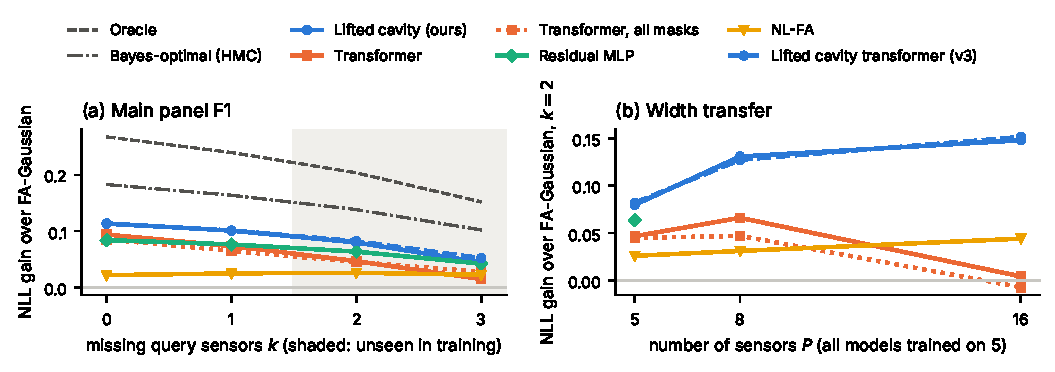
\includegraphics[width=\linewidth]{figures/main.pdf}
\caption{\label{fig:main}NLL gain over the closed-form FA-Gaussian anchor (higher is better). (a) Main panel F1 by
number of missing query sensors; shaded patterns were never seen in training. Grey lines are the privileged oracle and
the sign-conditioned HMC reference. (b) Width transfer with two missing sensors: every learned model was trained on five
sensors, and the residual MLP exists only at $P=5$. Dashed blue: the lifted cavity transformer of
\S\ref{sec:exp-v3}, descriptive on these panels.}
\end{figure}

Table~\ref{tab:main} and Figure~\ref{fig:main}a report the main panel. The lifted cavity network is the best
non-privileged method for every number of missing sensors, including the two- and three-sensor deletions it never saw
in training. With two missing sensors it closes \GapliftOne\% of the reference gap between FA-Gaussian and the
sign-conditioned HMC approximation. Two comparators close less: the residual MLP, which receives the same anchor and support
encodings with twice the parameters (\Gapanchormlp\%), and the tuned nonlinear plug-in model NL-FA (\Gapnlfa\%).
The TabPFN-v2-style transformer has 25 times the parameters and sees fresh tasks at every step. It is still worse
than the lifted cavity network at every number of missing sensors, by \MainkKZeroliftvspfnabs\ to
\MainkKTwoliftvspfnabs\ nats (all intervals exclude zero), and it closes \Gappfn\% of the gap. Training it on every
mask pattern does not change this (\Gappfnall\%): its deficit comes from how efficiently it learns fusion from a
finite training budget, not from unseen patterns. The residual MLP is the closest competitor in this setting. The
lifted cavity network beats it by \MainkKZeroliftvsmlpabs\ nats with all sensors observed and by
\MainkKTwoliftvsmlpabs\ with two missing, and the two tie with three missing.

EM-Gaussian, BLR and both ridges fall below FA-Gaussian; mean imputation is the worst of all.

\subsection{Generalization beyond the training distribution}
\label{sec:exp-shift}

\textbf{Width} (Table~\ref{tab:shift}, Figure~\ref{fig:main}b). The lifted cavity network runs unchanged on 8 and 16 sensors, where it improves on FA-Gaussian by
\SFTwogainfa\ \SFTwogainfaci\ and \SFThreegainfa\ \SFThreegainfaci\ nats with two missing sensors. The residual MLP
cannot run on these panels, and EM-Gaussian degrades as the covariance grows. The transformer also runs at any width, but it gains less over FA-Gaussian as sensors are added. On 16 sensors it is
no better than the closed form, and the lifted cavity network beats it by \SFThreegainpfn\ \SFThreegainpfnci\ nats.

\textbf{Support size.} With 16 calibration rows the transformer degrades sharply, while the lifted cavity network keeps
a \SFSixgainfa\ \SFSixgainfaci\ nat gain over FA-Gaussian; with 96 rows it remains the best method.
\textbf{Stronger nonlinearity} (0.8 instead of 0.4) is the one shift where the transformer competes. It ties the
lifted cavity network with two missing sensors (difference \XFFourkkTwoliftvspfn\ \XFFourkkTwoliftvspfnci) and is
better by \XFFourkkZeroliftvspfnabs\ nats when all sensors are observed: under strong response nonlinearity alone,
Gaussian re-linearization offers no advantage over a generic transformer.
\textbf{Linear sensors.} When the true sensors are linear, FA-Gaussian is nearly the right model and is best; the
learned re-linearization then costs \SFFivegainfaabs\ nats with two missing sensors, and the transformer
\XFFivekkTwopfnvsfaabs.

\subsection{What the lifting buys}
\label{sec:audit}

Ablations on F1 (Table~\ref{tab:ablation}, Appendix~\ref{app:more}) compare components of the small network. \textbf{Lifting} is the
largest factor: scalar sites ($K=0$) with otherwise identical machinery and training lose \AblLiftabs\ \AblLiftci\ nats
with two missing sensors and end up worse than the untrained FA-Gaussian anchor. This supports lifting empirically
under the tested training regime; Proposition~\ref{prop:scalar} does not cover this context-conditioned ablation.
\textbf{Cavity conditioning} adds \AblCavabs\ \AblCavci\ nats on top of lifted static sites. A second
nuisance dimension ($K=2$) changes nothing, as expected for one-factor noise. The scalar-cavity network of the earlier
design, retrained with the same 60{,}000-task recipe, remains far behind FA-Gaussian (Appendix~\ref{app:audit}).

\subsection{Real sensor networks}
\label{sec:exp-real}

\begin{table}[t]
\centering\scriptsize
\setlength{\tabcolsep}{2.5pt}
\caption{\label{tab:real}Real sensor networks: mean test NLL on later, held-out periods. Beijing: 12 target stations $\times$ weekly episodes in 2016--2017 with natural missingness, plus extra dropped sensors. Air Quality: weekly episodes after October 2004, sensor dropout simulated. Fine-tuning uses only earlier periods and one recipe for every model; lifted-cavity and residual-MLP rows average three seeds. Best entry per column in bold. $^\dagger$Post hoc. $^\ddagger$Designed after protocol v2 (Section~\ref{sec:exp-v3}); post hoc here and not bolded.}
\begin{tabular}{lccccccc}
\toprule
Method & \multicolumn{3}{c}{Beijing PM$_{2.5}$ (11 stations)} & \multicolumn{2}{c}{Air Quality CO} & \multicolumn{2}{c}{Air Quality NO$_2$}\\
 & natural & $+3$ & $+6$ & $k{=}0$ & $k{=}2$ & $k{=}0$ & $k{=}2$\\
\midrule
EM-Gaussian & 1.032 & 0.742 & 0.569 & 0.074 & 0.085 & $-$0.237 & $-$0.175\\
FA-Gaussian & 0.677 & 0.615 & 0.562 & 0.052 & 0.116 & $-$0.196 & $-$0.155\\
NL-FA & 0.938 & 0.744 & 0.610 & 0.144 & 0.091 & $-$0.090 & $-$0.142\\
Bayesian linear regression & 0.399 & 0.406 & 0.442 & 1.037 & 0.216 & $-$0.055 & $-$0.178\\
Ridge (complete case) & 0.425 & 0.432 & 0.458 & 0.824 & 0.208 & $-$0.200 & $-$0.176\\
GP, complete case$^\dagger$ & 1.884 & 1.312 & 0.934 & 3.364 & 0.503 & 25.217 & $-$0.198\\
$k$-nearest neighbours$^\dagger$ & 0.508 & 0.514 & 0.540 & 0.571 & 0.353 & $-$0.010 & $-$0.063\\
\midrule
Lifted cavity, zero-shot & 0.826 & 0.661 & 0.561 & 0.044 & 0.129 & $-$0.350 & $-$0.233\\
Transformer, zero-shot & 0.958 & 0.743 & 0.687 & $-$0.017 & 0.081 & $-$0.360 & $-$0.231\\
\midrule
\textbf{Lifted cavity, fine-tuned (ours)} & 0.205 & 0.237 & 0.305 & $-$0.040 & 0.008 & $-$0.412 & $-$0.337\\
\quad no synthetic pretraining & 0.247 & 0.279 & 0.344 & $-$0.001 & $-$0.006 & $-$0.419 & $-$0.316\\
\quad no cavity input & 0.259 & 0.286 & 0.349 & $-$0.086 & $-$0.028 & $-$0.423 & $-$0.332\\
\quad scalar sites ($K=0$) & 0.215 & 0.252 & 0.347 & $-$0.026 & $-$0.003 & $-$0.359 & $-$0.302\\
Transformer, fine-tuned & \textbf{0.087} & \textbf{0.121} & \textbf{0.236} & \textbf{$-$0.163} & \textbf{$-$0.052} & \textbf{$-$0.485} & \textbf{$-$0.381}\\
Residual MLP, fine-tuned & -- & -- & -- & 0.025 & 0.110 & $-$0.246 & $-$0.147\\
\emph{Lifted cavity transformer, fine-tuned}$^\ddagger$ & 0.122 & 0.160 & 0.259 & $-$0.099 & $-$0.027 & $-$0.404 & $-$0.359\\
\bottomrule
\end{tabular}
\end{table}


\paragraph{Beijing multi-site air quality~\citep{zhang2017beijing}.}
The task is to predict log PM$_{2.5}$ at each of 12 monitoring stations from the other 11, using hourly data with
natural missingness. This tests contemporaneous missing-station interpolation, rather than low-cost-device calibration
or future forecasting. Each episode is one station and one week, with 48 labeled support hours and 48 query hours. The
test period (2016-01 to 2017-02, \Rbeijingepisodes\ episodes) was never examined before protocol v2 was committed.
Learned models are fine-tuned on episodes from 2013--2015 with one fixed recipe; the protocol's analysis is
cluster-robust over weeks.

With 11 sensors and 48 rows, the joint-covariance closed forms overfit, and evidence-tuned BLR is the strongest closed
form. The fine-tuned lifted cavity network improves on it by \RbeijingeZerovsblrabs\ \RbeijingeZerovsblrci\ nats under
natural missingness, and by \RbeijingeSixvsblrabs\ \RbeijingeSixvsblrci\ with six further sensors removed.
The fine-tuned transformer is better still. The lifted cavity network's gain over it is \RbeijingeZerovspfn\
\RbeijingeZerovspfnci\ nats under natural missingness and \RbeijingeSixvspfn\ \RbeijingeSixvspfnci\ with six sensors
removed, so endpoint E4b fails. Before fine-tuning the order is reversed: zero-shot, the lifted cavity network is ahead
by \RbeijingeSixzsliftvspfnabs\ \RbeijingeSixzsliftvspfnci\ nats with six sensors removed. Fine-tuning improves the
transformer by more than it improves the lifted network (Table~\ref{tab:real}).

Synthetic pretraining helps: the same network fine-tuned from initialization is \RbeijingeZerovsnopreabs\ nats
worse \RbeijingeZerovsnopreci.

\paragraph{UCI Air Quality~\citep{devito2008airquality}.}
Five metal-oxide sensors on one device predict the reference analyzers' log CO and log NO$_2$, in weekly episodes
after October 2004. These weeks were examined in protocol v1, so this is secondary evidence.
With two simulated missing sensors, the fine-tuned lifted cavity network improves on FA-Gaussian by
\RairqcoeTwovsfa\ \RairqcoeTwovsfaci\ nats for CO and \RairqnoTwoeTwovsfa\ \RairqnoTwoeTwovsfaci\ for NO$_2$. The
fine-tuned transformer is again better: the lifted network's gain over it is \RairqcoeTwovspfn\ \RairqcoeTwovspfnci\
(CO) and \RairqnoTwoeTwovspfn\ \RairqnoTwoeTwovspfnci\ (NO$_2$). On CO, the cavity input stops helping after
fine-tuning.

\paragraph{Why the transformer wins on real data.}
The lifted network underfits rather than overfits: on the Beijing fine-tuning episodes, the transformer's final
training NLL is \FTbeijingtraingap\ nats lower, about the size of the test gap. Post-hoc variants do not close the gap
on Beijing (Table~\ref{tab:explore}; natural missingness, transformer \RbeijingeZerovalftpfn): a second nuisance dimension scores \Xplifttwo\
and five times more fine-tuning steps \Xpliftlong, against \Xpliftone\ for the same seed with the standard recipe.
Nor is the edge that of a flexible per-episode regression: a Gaussian process fitted to each episode's calibration
rows is the worst method on Air Quality (\RairqcoeZerovalgp\ nats for CO with all sensors observed). These point to
the Gaussian site family itself. Gaussian sites with per-sensor re-linearization are a strong prior for synthetic
factor noise, but real stations share structure they cannot express, and a generic model learns it from a few
thousand real episodes: fine-tuning improves the transformer by \FTbeijingpfngain\ nats on Beijing and the lifted
network by \FTbeijingliftgain.


\subsection{Lifted sites as a transformer output layer (protocol v3)}
\label{sec:exp-v3}

Protocol v2 left a split: structure wins on synthetic tasks, the transformer on real networks after fine-tuning. The
\emph{lifted cavity transformer} (LCT; \S\ref{sec:method-lct}) keeps the transformer's backbone, recipe and seed, with
a lifted probabilistic readout. Because the hypothesis was formed after the v2 results, v3 uses new panels (G1,
five sensors; G3, sixteen) and two Beijing pollutants never scored before (NO$_2$ and CO), and its four endpoints were
committed before any of these existed (Table~\ref{tab:endpoints}).

\begin{table}[t]
\centering\scriptsize
\setlength{\tabcolsep}{3pt}
\caption{\label{tab:v3}Protocol v3 (new panels and targets). Mean test NLL. G1: 256 fresh five-sensor tasks by number of missing query sensors $k$; G3: 128 fresh 16-sensor tasks, $k=2$. Beijing: log NO$_2$ and log CO at each station from the other 11 stations, 2016--2017, natural missingness and six further sensors removed; learned models fine-tuned with the recipe of protocol v2 (the all-mask transformer was not fine-tuned). Best entry per column in bold.}
\begin{tabular}{lccccccccc}
\toprule
 & \multicolumn{4}{c}{G1, $P{=}5$} & G3 & \multicolumn{2}{c}{Beijing NO$_2$} & \multicolumn{2}{c}{Beijing CO}\\
Method & $k{=}0$ & $k{=}1$ & $k{=}2$ & $k{=}3$ & $P{=}16$ & natural & $+6$ & natural & $+6$\\
\midrule
FA-Gaussian & \textbf{$-$0.189} & \textbf{$-$0.054} & \textbf{0.129} & \textbf{0.396} & \textbf{$-$0.806} & 0.684 & 0.506 & -- & --\\
Bayesian linear regression & 0.013 & 0.022 & 0.153 & 0.401 & 0.063 & \textbf{0.275} & \textbf{0.365} & -- & --\\
\midrule
Lifted cavity network, 8k & -- & -- & -- & -- & -- & -- & -- & -- & --\\
Transformer, 203k & -- & -- & -- & -- & -- & -- & -- & -- & --\\
Transformer, all masks, 203k & -- & -- & -- & -- & -- & -- & -- & -- & --\\
\textbf{Lifted cavity transformer}, 203k & -- & -- & -- & -- & -- & -- & -- & -- & --\\
\bottomrule
\end{tabular}
\end{table}


\noindent On the fresh synthetic panels, the lifted output layer helps the transformer (Table~\ref{tab:v3}). With two
missing sensors the LCT beats the transformer with the identical backbone, recipe and seed by
\VthreeGOnekTwolctvspfnabs\ \VthreeGOnekTwolctvspfnci\ nats on G1 and \VthreeGThreekTwolctvspfnabs\
\VthreeGThreekTwolctvspfnci\ on sixteen sensors (E5, E6 pass). It matches the small lifted network on five sensors
(\VthreeGOnekTwolctvslift\ \VthreeGOnekTwolctvsliftci) and exceeds it on sixteen (\VthreeGThreekTwolctvslift\
\VthreeGThreekTwolctvsliftci), and it learns faster: its training NLL reaches the transformer's final value after
\Trainlctreach\ of 30{,}000 steps (Figure~\ref{fig:training}). On the v2 panels (descriptive) it closes \Gaplct\% of
the F1 gap (lifted network \GapliftOne\%) but inherits part of the transformer's degradation with 16 calibration rows.
After fine-tuning on Beijing NO$_2$, it beats the fine-tuned lifted network by \VthreebeijingnoTwoeZerolctvslift\
\VthreebeijingnoTwoeZerolctvsliftci\ nats (E7a passes), recovering \VthreebeijingnoTwoeZerorecovered\% of the gap
between the lifted network (\VthreebeijingnoTwoeZerovallift) and the transformer (\VthreebeijingnoTwoeZerovalpfn).
Against the transformer the difference is \VthreebeijingnoTwoeZerolctvspfn\ \VthreebeijingnoTwoeZerolctvspfnci; the
interval includes zero but extends below the margin of $-0.02$, so non-inferiority (E7b) is not established. With six
more stations missing, the two tie (\VthreebeijingnoTwoeSixlctvspfn\ \VthreebeijingnoTwoeSixlctvspfnci).
\input{exp_v3_co}




\subsection{Pre-registered endpoints and calibration}
\label{sec:exp-endpoints}

Table~\ref{tab:endpoints} lists every pre-registered endpoint of protocols v2 and v3. Five of six v2 endpoints pass;
the failure, E4b, is the real-data comparison with the fine-tuned transformer. All five v1 endpoints passed
(Appendix~\ref{app:audit}). Three of the four v3 endpoints pass; the failure, E7b, is non-inferiority to the fine-tuned transformer on Beijing
NO$_2$, where the interval is wide.
 Learned models are close to nominal 90\% coverage (lifted
cavity network \CalliftOneFcov\ on F1, \CalliftOneBcov\ on Beijing), while the closed forms under-cover
(Table~\ref{tab:calib}).

